\setRL
\pagenumbering{arabic} 


\section{
غشای زیستی
}
با پیشرفت تکنولوژی میکروسکوپ،‌ امروزه با تصاویری از سلول روبرو هستیم که شامل جزئیات و پیچیدگی‌های بسیار زیادی است. به علت زحمات افراد در قرن ۱۹ میلادی برای پی بردن به ساز و کار واحد‌های سازنده‌ی موجودات زنده، ما امروز می‌دانیم که غشای زیستی لایه‌ی نازکی است که تمام سلول‌های زنده را می‌پوشاند. این لایه ارتباط سلول با محیط اطراف را کنترل و مدیریت می‌کند. غشای زیستی از ملکول‌های چربی
\LTRfootnote{lipid}  
با یک سر آب دوست
\LTRfootnote{hydrophilic}  
 و یک دُم آب گریز
 \LTRfootnote{hydrophobic}  
 ساخته شده‌است (شکل
\ref{fig:phospholipid}
).
 
 \begin{figure}[h]
\begin{center}
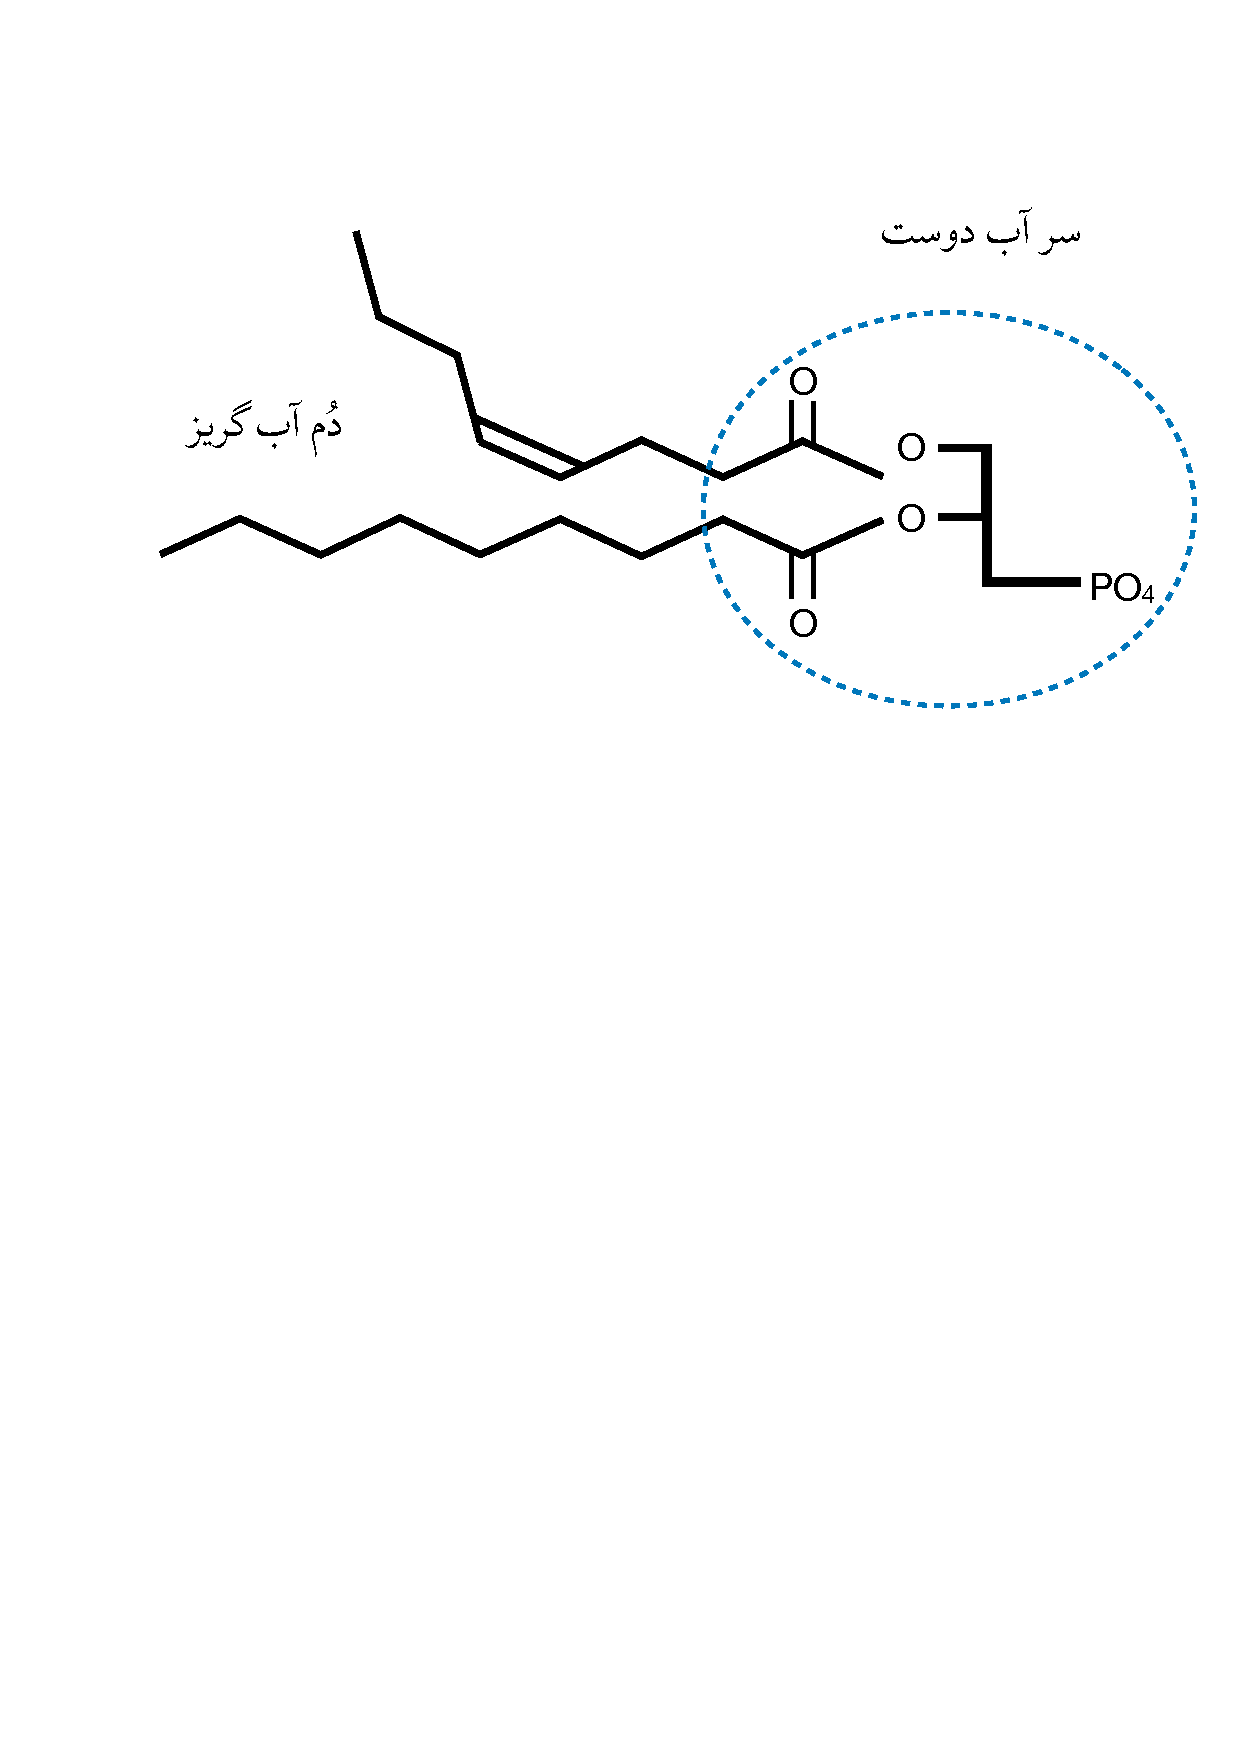
\includegraphics[width=4in]{\MemBio /Pics/Phospholipid}
\caption{
ساختار شیمیایی یک ملکول فوسفولیپید. سر آب دوست (دایره‌ی آبی) و  انتهای آبگریز مشخص شده است.
}
\label{fig:phospholipid}
\end{center}
\end{figure}
 
 
  وجود این دو سر باعث می‌شود که این ملکول‌ها در محلول‌های آبی
\textbf{بدون ایجاد پیوندها شیمیایی}
، به طور خود سامانده
  \LTRfootnote{self-assembly}  
 سطوح بزرگ تشکیل دهند. این سطوح اقلب از دو لایه ملکول چرب تشکیل شده که دُم‌های  آبگریز در مرکز لایه (و به دور از آب) قرار دارد (شکل
\ref{fig:bilayer}
 ).
\begin{figure}[h]
\begin{center}
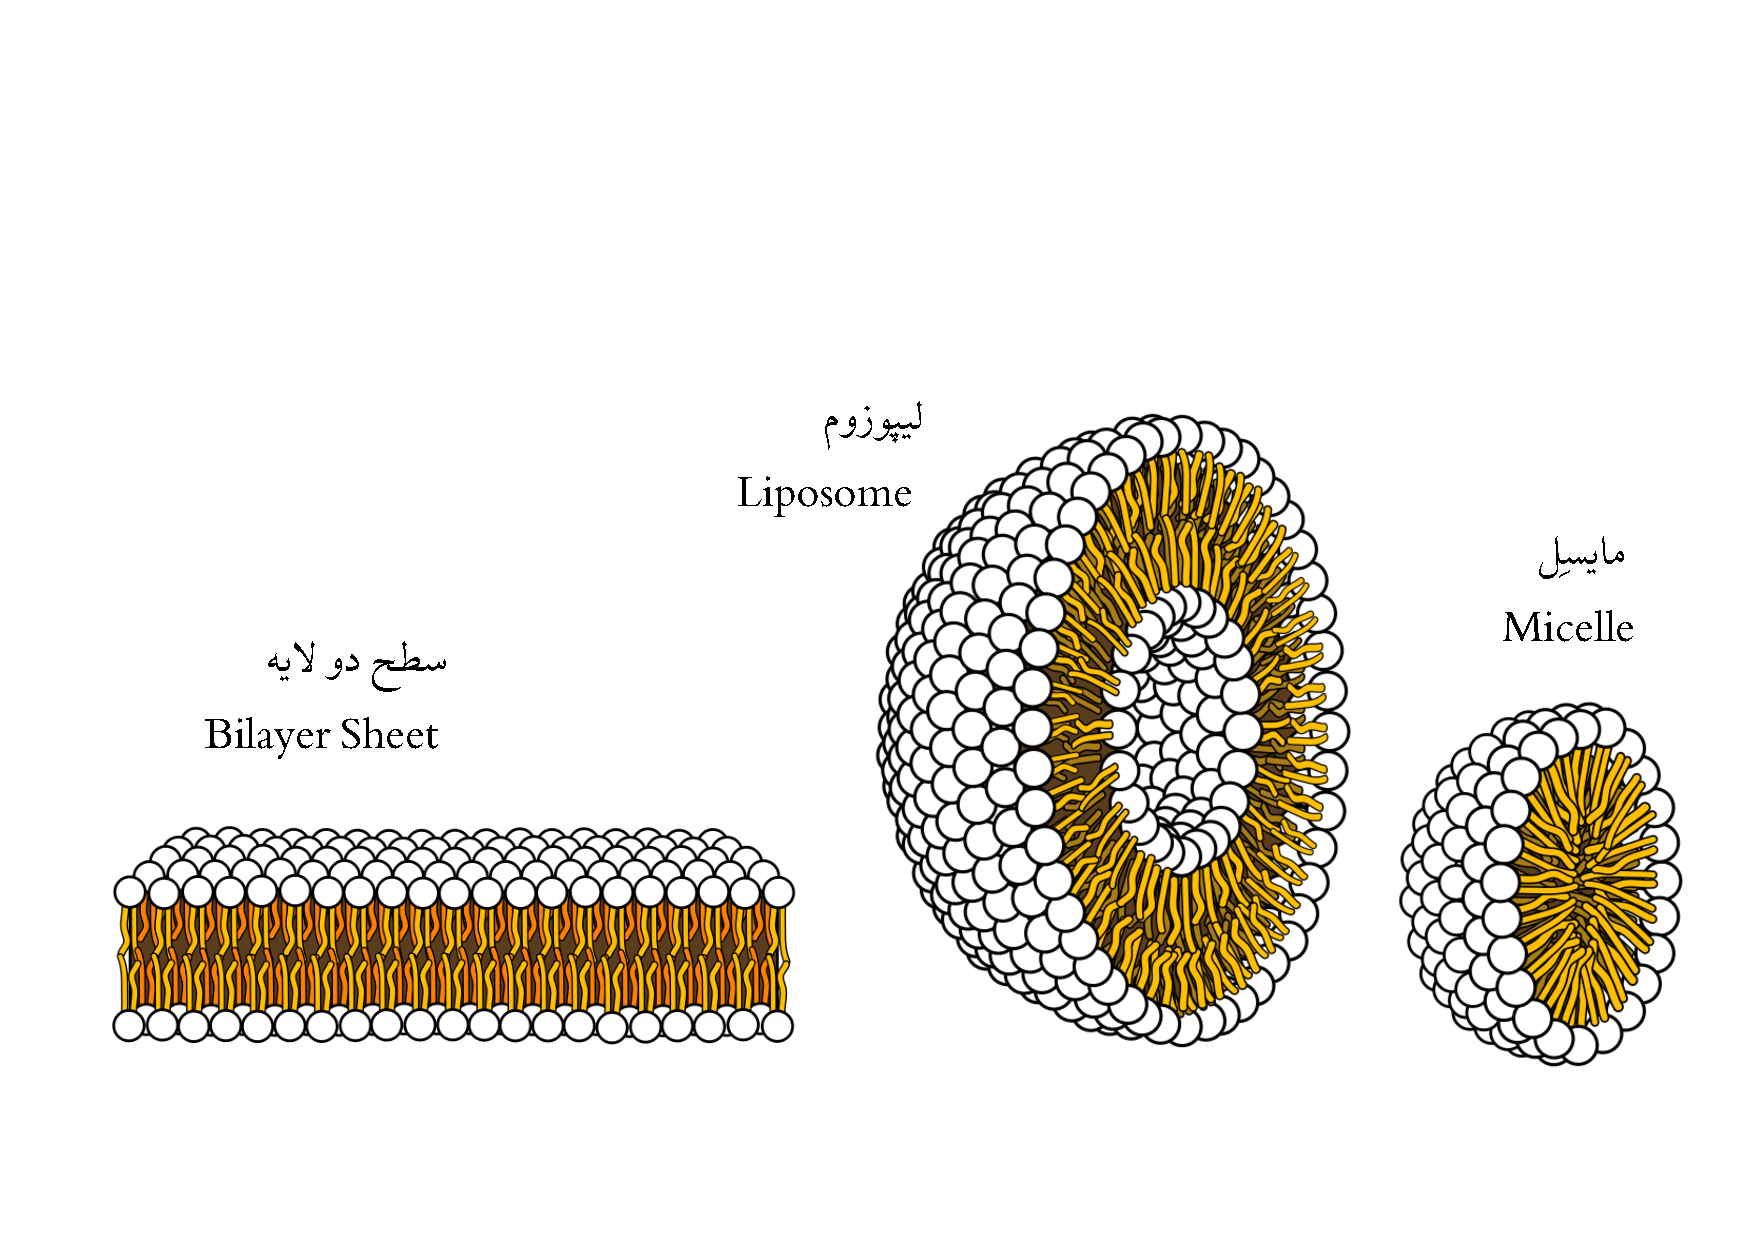
\includegraphics[width=4in]{\MemBio /Pics/Bilayer}
\caption{
ساختار‌های معمول ملکول‌های چربی در آب. به ترتیب از چپ به راست، ساختار سطوح بزرگ دو لایه، کره‌های دو لایه (لیپوزوم)، و کره‌های کوچک تک لایه، مایسِل.
}
\label{fig:bilayer}
\end{center}
\end{figure}
 
 
 
 
 
 
 
 
 
 
 
 
 
 
 
 
 
 
 